
\documentclass[conference]{IEEEtran}
\usepackage{graphicx}
\usepackage{amsmath}
\usepackage{booktabs}
\usepackage{array}
\usepackage{url}
\usepackage{cite}
\usepackage{float}
\usepackage{xcolor}
\usepackage{tikz}
\usetikzlibrary{positioning,shapes.geometric,arrows.meta}

\title{Customer Churn Prediction Using Machine Learning and an Interactive Streamlit Dashboard}

\author{\IEEEauthorblockN{Zunaira Tahir}
\IEEEauthorblockA{BSc Artificial Intelligence\\
AI \& Machine Learning Internship\\
IT Simplera Solutions}}

\begin{document}
\maketitle

\begin{abstract}
Customer churn is a significant challenge for telecommunication companies because losing existing customers can reduce revenue and increase customer acquisition costs. This paper presents an end-to-end machine learning system for predicting customer churn using the Iranian Churn Dataset from the UCI Machine Learning Repository. The workflow includes data inspection, preprocessing, exploratory analysis, feature preparation, baseline classification, Random Forest optimization, error analysis, and deployment. Several classification models were investigated, with Random Forest selected as the final model after hyperparameter tuning. The study also considers explainable artificial intelligence to improve the interpretation of churn predictions and to connect model outputs with customer-retention decisions. The optimized model was integrated into an interactive Streamlit dashboard that allows users to enter customer information and obtain an immediate churn prediction. The resulting system demonstrates a practical pipeline from raw customer data to a deployable prediction application. The work highlights the value of combining predictive machine learning, model evaluation, interpretability, and lightweight web deployment for customer-retention support in telecommunications.
\end{abstract}

\begin{IEEEkeywords}
Customer churn, machine learning, Random Forest, explainable AI, telecommunications, Streamlit, customer retention.
\end{IEEEkeywords}

\section{Introduction}
Customer churn refers to the situation in which a customer stops using a company's service. In telecommunications, churn is particularly important because customer acquisition is expensive and small changes in retention can have a substantial effect on long-term revenue. The increasing availability of customer usage, service, demographic, and value-related data creates an opportunity to identify customers who are more likely to leave before churn occurs.

Machine learning is widely used for churn prediction because it can learn relationships between customer attributes and a binary churn outcome. Recent studies have investigated decision trees, Random Forest, gradient boosting, support vector machines, k-nearest neighbors, and ensemble approaches. In addition to predictive performance, recent work increasingly emphasizes explainability because business users need to understand why a customer has been classified as high risk \cite{poudel2024,atay2025,liu2025}.

This work develops a complete customer churn prediction workflow using the Iranian Churn Dataset. The project covers data preprocessing, exploratory data analysis, model development, model comparison, hyperparameter tuning, error analysis, and deployment through Streamlit. The central practical objective is not only to train a classifier but also to convert the trained model into a usable prediction interface.

The main contributions are:
\begin{itemize}
\item preparation and analysis of telecom customer data for churn classification;
\item comparison of multiple supervised learning approaches;
\item optimization of a Random Forest classifier;
\item analysis of prediction errors and model behavior;
\item consideration of explainable machine learning for interpretation; and
\item deployment of the final model through an interactive Streamlit dashboard.
\end{itemize}

\section{Related Work}
Recent churn research demonstrates that machine learning can provide effective early-warning systems for telecom operators. Poudel et al. studied tabular machine learning models and emphasized the importance of explaining both global and local churn predictions. Their work reported strong performance from gradient boosting and used SHAP-based explanations to identify influential predictors \cite{poudel2024}.

A 2024 study on telecom churn compared Random Forest, k-nearest neighbors, and decision-tree based approaches and reported very strong Random Forest performance, demonstrating the usefulness of ensemble tree models for churn classification \cite{telecom2024}. Sikri et al. similarly investigated machine-learning driven churn prediction with an emphasis on customer-retention decisions \cite{sikri2024}.

Atay and Turanli specifically analyzed the UCI Iranian Churn dataset using logistic regression, k-nearest neighbors, decision trees, and Random Forest. Their results showed that a tuned Random Forest achieved an accuracy of 0.9562 and an AUC of 0.9042, with complaints identified as an important predictor \cite{atay2025}. This study is particularly relevant because it uses the same public dataset as the present work.

More recent research has extended the Iranian Churn benchmark with explainability and extensive hyperparameter tuning. A 2025 conference study trained seven machine-learning models on the Iranian Churn dataset and reported strong CatBoost performance after tuning, while using SHAP for global and local interpretation \cite{liu2025}. Other recent work has explored heterogeneous stacking, class-imbalance handling, and explainable counterfactual analysis \cite{hmse2024,counterfactual2025}.

Table~\ref{tab:related} summarizes the five core papers reviewed for this study.

\begin{table}[H]
\centering
\caption{Summary of reviewed research}
\label{tab:related}
\small
\begin{tabular}{p{1.8cm}p{0.65cm}p{2.0cm}p{2.0cm}}
\toprule
Study & Year & Main focus & Identified gap \\
\midrule
Poudel et al. & 2024 & Tabular ML and SHAP explanations & Deployment not central \\
Telecom ML study & 2024 & RF, KNN and DT comparison & Limited interpretability \\
Sikri et al. & 2024 & ML-based retention support & Dataset/model dependence \\
Atay \& Turanli & 2025 & Tuned RF on Iranian Churn & Limited application deployment \\
Liu & 2025 & Tuned models and SHAP & Greater complexity than lightweight deployment \\
\bottomrule
\end{tabular}
\end{table}

The reviewed literature suggests three recurring gaps: first, many studies focus primarily on predictive scores; second, model interpretability is not always integrated with practical decision support; and third, the final model is often evaluated without demonstrating a lightweight user-facing deployment. The present project addresses the third gap directly and combines it with model optimization and interpretability-oriented analysis.

\clearpage
\section{Dataset}
The study uses the Iranian Churn Dataset provided by the UCI Machine Learning Repository. The dataset contains 3,150 customer records and 13 input features, with a binary churn target. The data was collected from an Iranian telecommunications company over a 12-month period. Customer attributes include call failures, complaints, subscription length, charge amount, seconds of use, frequency of use, frequency of SMS, distinct called numbers, age group, tariff plan, status, age, and customer value \cite{uci2020}.

The dataset is a binary classification problem. The UCI documentation states that the customer attributes are aggregated from the first nine months, while the churn status is determined at the end of the 12-month period, leaving a three-month planning gap. This temporal design makes the dataset suitable for an early churn prediction setting \cite{uci2020}.

\subsection{Preprocessing}
The preprocessing workflow consisted of data loading, structural inspection, data-type checking, missing-value inspection, duplicate checking, exploratory analysis, feature-target separation, and preparation of numerical/categorical representations for model training. The target variable was separated from the explanatory features before model fitting.

The project also included visualization of feature distributions and relationships, correlation analysis, and inspection of churn-related patterns. These steps were used to understand the data before training and to reduce the risk of applying inappropriate transformations.

\clearpage
\section{Methodology}
The proposed workflow follows a standard supervised learning pipeline:

\begin{figure}[H]
\centering
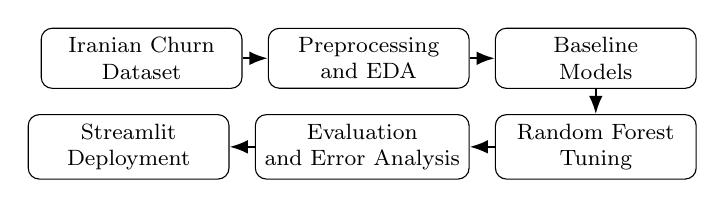
\begin{tikzpicture}[
node distance=0.32cm,
box/.style={draw, rounded corners, align=center, minimum width=2.55cm, minimum height=0.55cm, font=\footnotesize},
arr/.style={-{Latex}, thick}
]
\node[box] (data) {Iranian Churn\\Dataset};
\node[box, right=of data] (prep) {Preprocessing\\and EDA};
\node[box, right=of prep] (models) {Baseline\\Models};
\node[box, below=of models] (tune) {Random Forest\\Tuning};
\node[box, left=of tune] (eval) {Evaluation\\and Error Analysis};
\node[box, left=of eval] (deploy) {Streamlit\\Deployment};
\draw[arr] (data)--(prep);
\draw[arr] (prep)--(models);
\draw[arr] (models)--(tune);
\draw[arr] (tune)--(eval);
\draw[arr] (eval)--(deploy);
\end{tikzpicture}
\caption{End-to-end workflow of the proposed customer churn prediction system.}
\end{figure}

\subsection{Baseline Models}
Multiple supervised classification algorithms were considered as baselines. Logistic Regression provides a simple linear decision boundary and is useful as an interpretable reference. Decision Tree classification provides nonlinear decision rules, while Random Forest combines multiple decision trees to improve robustness and reduce the variance of an individual tree.

\subsection{Random Forest Optimization}
Random Forest was selected for further improvement because ensemble tree models are well suited to heterogeneous tabular customer data and have demonstrated strong performance in telecom churn research. Hyperparameter tuning was used to search for a better combination of model settings. The tuned model was then used as the final predictive component of the application.

\subsection{Explainability}
Explainable AI is important for churn prediction because a binary label alone does not explain the business reason behind a prediction. SHAP is a model-agnostic explanation framework commonly used to estimate the contribution of individual features to predictions \cite{lundberg2017}. In this project, explainability is treated as an interpretive layer that can help connect customer attributes with model decisions.

\section{Experimental Setup}
The experiments were conducted in Python using standard data-science and machine-learning libraries. Pandas and NumPy were used for data handling, Matplotlib and Seaborn for visualization, and Scikit-learn for model training and evaluation. Joblib was used to save the final trained model, while Streamlit was used for deployment.

The dataset was divided into training and testing subsets. Model performance was assessed using classification metrics including accuracy, precision, recall, F1-score, and confusion-matrix analysis. The evaluation process was designed to compare baseline approaches with the optimized Random Forest model.

For reproducibility, the project keeps the preprocessing, model-development notebooks, saved model, and deployment source code together. The final application accepts the same feature structure used during model training so that the deployment interface remains consistent with the training pipeline.

\clearpage
\section{Results}
The project successfully produced a complete churn prediction workflow and an interactive dashboard. During model development, multiple classifiers were evaluated and Random Forest was selected for optimization. The tuned Random Forest became the final model used by the deployed application.

\begin{table}[H]
\centering
\caption{Model comparison in the project workflow}
\label{tab:models}
\small
\begin{tabular}{p{2.3cm}p{2.0cm}p{2.3cm}}
\toprule
Model & Role & Project outcome \\
\midrule
Logistic Regression & Baseline linear model & Evaluated \\
Decision Tree & Nonlinear baseline & Evaluated \\
Random Forest & Ensemble model & Selected for tuning \\
Tuned Random Forest & Final model & Used for deployment \\
\bottomrule
\end{tabular}
\end{table}

Because the purpose of the project was both predictive modeling and deployment, the final result was evaluated at two levels: predictive modeling and practical usability. At the modeling level, tuning was used to improve the selected Random Forest configuration. At the application level, the trained model was successfully integrated into a Streamlit dashboard where a user can enter customer information and receive a churn prediction.

\begin{figure}[H]
\centering
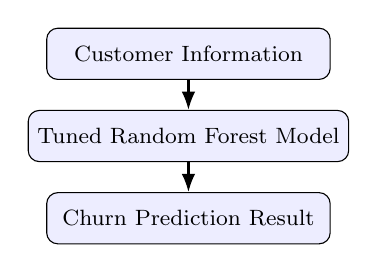
\begin{tikzpicture}[
node distance=0.38cm,
box/.style={draw, rounded corners, align=center, minimum width=3.6cm, minimum height=0.65cm, font=\footnotesize, fill=blue!7},
arr/.style={-{Latex}, thick}
]
\node[box] (input) {Customer Information};
\node[box, below=of input] (model) {Tuned Random Forest Model};
\node[box, below=of model] (result) {Churn Prediction Result};
\draw[arr] (input) -- (model);
\draw[arr] (model) -- (result);
\end{tikzpicture}
\caption{Deployment flow from customer inputs to the final churn prediction.}
\end{figure}

\clearpage
\section{Discussion}
The project demonstrates that customer churn prediction can be implemented as a complete pipeline rather than as an isolated model-training exercise. The use of Random Forest is consistent with recent research, which repeatedly identifies tree-based ensembles as strong candidates for telecom churn data \cite{poudel2024,atay2025}. Hyperparameter tuning provides an additional opportunity to adapt the model to the selected dataset rather than relying only on default parameters.

The deployment component is an important practical contribution. A trained model has limited operational value if it cannot be accessed by a non-technical user. The Streamlit interface converts the model into a simple application in which customer attributes are entered and a prediction is returned immediately.

Several limitations should be acknowledged. First, the model is trained on a single public telecom dataset collected from one company and therefore may not generalize to other operators or countries. Second, churn is a behavioral outcome and may be influenced by factors not represented in the dataset, such as competitor offers, network quality, customer support interactions, pricing changes, and external market conditions. Third, explainability does not automatically establish causality: a feature that strongly influences a model prediction should not be interpreted as a proven cause of churn.

Failure cases are also important. False negatives are particularly costly because a customer who is predicted as non-churning may leave without receiving a retention intervention. Future versions should therefore consider probability calibration, threshold optimization, class-imbalance strategies, and cost-sensitive learning.

\clearpage
\section{Conclusion and Future Work}
This paper presented an end-to-end customer churn prediction system based on machine learning and an interactive Streamlit dashboard. The workflow covered dataset preparation, exploratory analysis, classification model development, Random Forest optimization, evaluation, error analysis, explainability considerations, and deployment.

The final system demonstrates how a machine-learning model can be transformed into a practical customer-retention support tool. Instead of providing only an offline prediction, the deployed application allows customer information to be entered interactively and produces an immediate churn prediction.

Future work can extend the system in several directions. First, additional telecom datasets should be evaluated to test generalization. Second, class-imbalance techniques such as SMOTE and cost-sensitive learning can be investigated where appropriate. Third, probability calibration and threshold optimization can be used to better prioritize high-risk customers. Fourth, SHAP-based global and local explanations can be integrated directly into the dashboard. Finally, future deployments could incorporate real-time customer data, monitoring, model drift detection, and retention recommendations.

\begin{thebibliography}{00}

\bibitem{uci2020}
UCI Machine Learning Repository, ``Iranian Churn Dataset,'' 2020, doi: 10.24432/C5JW3Z.

\bibitem{poudel2024}
S. Sharma Poudel, S. Pokharel, and M. Timilsina, ``Explaining customer churn prediction in telecom industry using tabular machine learning models,'' \emph{Machine Learning with Applications}, vol. 17, 100567, 2024, doi: 10.1016/j.mlwa.2024.100567.

\bibitem{telecom2024}
``Customer churn prediction in telecom sector using machine learning techniques,'' \emph{Results in Control and Optimization}, vol. 14, 100342, 2024, doi: 10.1016/j.rico.2023.100342.

\bibitem{sikri2024}
A. Sikri, R. Jameel, S. M. Idrees, and H. Kaur, ``Enhancing customer retention in telecom industry with machine learning driven churn prediction,'' \emph{Scientific Reports}, vol. 14, 13097, 2024, doi: 10.1038/s41598-024-63750-0.

\bibitem{atay2025}
M. T. Atay and M. Turanli, ``Analysis of customer churn prediction using logistic regression, k-nearest neighbors, decision tree and random forest algorithms,'' \emph{Advances and Applications in Statistics}, vol. 92, no. 2, pp. 147--169, 2025, doi: 10.17654/0972361725008.

\bibitem{liu2025}
Z. Liu, ``Telecom customer churn prediction with explainable machine learning,'' in \emph{Proc. 2nd Int. Conf. Modeling, Natural Language Processing and Machine Learning}, 2025, doi: 10.1145/3757110.3757152.

\bibitem{hmse2024}
``Sampling-based novel heterogeneous multi-layer stacking ensemble method for telecom customer churn prediction,'' 2024, \emph{Results in Engineering}.

\bibitem{counterfactual2025}
``Ensemble counterfactual explanations for churn analysis,'' in \emph{Springer Lecture Notes in Computer Science}, 2025.

\bibitem{lundberg2017}
S. M. Lundberg and S.-I. Lee, ``A unified approach to interpreting model predictions,'' in \emph{Advances in Neural Information Processing Systems}, vol. 30, 2017.

\bibitem{breiman2001}
L. Breiman, ``Random forests,'' \emph{Machine Learning}, vol. 45, pp. 5--32, 2001.

\end{thebibliography}

\end{document}
